\documentclass[12pt]{article}

% -------------------- Packages --------------------
\usepackage{hyperref}
\usepackage{listings}
\usepackage[margin=1in]{geometry}
\usepackage{enumitem}
\usepackage{array}
\usepackage{titlesec}
\usepackage{helvet}
\renewcommand{\familydefault}{\sfdefault}

% Math packages
\usepackage{amsmath}     % For math equations
\usepackage{amssymb}     % For advanced math symbols
\usepackage{amsfonts}    % For math fonts
\usepackage{gvv}         % Custom matrix/vector formatting
\usepackage{esint}

% Other packages
\usepackage[utf8]{inputenc}
\usepackage{graphicx}
\usepackage{pgfplots}
\pgfplotsset{compat=1.18}
\usepackage{multirow}
\usepackage{float}
\usepackage{caption}
\usepackage{multicol}

% -------------------- Formatting --------------------
\titleformat{\section}{\bfseries\large}{\thesection.}{1em}{}
\setlength{\parindent}{0pt}
\setlength{\parskip}{6pt}
\renewcommand{\labelenumi}{\alph{enumi})}

% -------------------- Document --------------------
\begin{document}

\newpage
\begin{center}
\textbf{\Large AI25BTECH11034 - SUJAL CHAUHAN }\\
\textbf{4.8.30}
\end{center}

\textbf{Question:}\\
Find the equation of a line passing through the point (2,3,2) and parallel to the line \\
$\Vec{r}= (-2\hat{i}+3\hat{j})+\lambda(2\hat{i}-3\hat{j}+6\hat{k})$. Also, find the distance beteween these two lines.\\[2cm]

\textbf{Theory:}  

Consider two parallel lines in 3D:
\begin{align}
    \vec{r}_1 &= \vec{a}_1 + \lambda \vec{b}, \quad \lambda \in \mathbb{R}, \\[6pt]
    \vec{r}_2 &= \vec{a}_2 + \mu \vec{b}, \quad \mu \in \mathbb{R},
\end{align}
where $\vec{a}_1, \vec{a}_2$ are points on the respective lines and $\vec{b}$ is the common direction vector.  

The vector $\vec{a}_2 - \vec{a}_1$ lies in the plane spanned by $\{\vec{a}_2 - \vec{a}_1, \vec{b}\}$.  
To find the shortest distance between the lines, we first determine a vector $\vec{n}$ that is orthogonal to both:
\begin{align}
    \vec{n}^T \myvec{ \vec{a}_2 - \vec{a}_1 & \vec{b} } = \vec{0}.
\end{align}

Solving this system yields an orthogonal vector $\vec{n}$.  
Then, the shortest distance $d$ between the two parallel lines is the orthogonal projection of $(\vec{a}_2 - \vec{a}_1)$ onto the direction of $\vec{n}$:
\begin{align}
    d &= \frac{(\vec{a}_2 - \vec{a}_1)^T \vec{n} }{\|\vec{n}\|}.
\end{align}


\textbf{Solution:}\\[2cm]
The direction vector of the given parallel lines is
\begin{align}
    \vec{b} = \myvec{2 \\ -3 \\ 6}.
\end{align}

The first line is given by
\begin{align}
    \vec{r}_1 = \myvec{2 \\ 3 \\ 2} + \mu \myvec{2 \\ -3 \\ 6}, \quad \mu \in \mathbb{R}.
\end{align}

The second line is
\begin{align}
    \vec{r}_2 = \myvec{-2 \\ 3 \\ 0} + \lambda \myvec{2 \\ -3 \\ 6}, \quad \lambda \in \mathbb{R}.
\end{align}

Now, the difference between the two given points on the lines is
\begin{align}
    \vec{a}_2 - \vec{a}_1 
    = \myvec{-2 \\ 3 \\ 0} - \myvec{2 \\ 3 \\ 2} 
    = \myvec{4 \\ 0 \\ 2}.
\end{align}

To find the shortest distance, we first compute a vector $\vec{n}$ orthogonal to both $\vec{b}$ and $\vec{a}_2 - \vec{a}_1$.  
This requires solving
\begin{align}
    \vec{n}^T 
    \myvec{
        2 & 4 \\
       -3 & 0 \\
        6 & 2
    } = \vec{0}.
\end{align}

On solving, we obtain
\begin{align}
    \vec{n} = k \myvec{-3 \\ 2 \\ 2}, \quad k \in \mathbb{R}.
\end{align}

Finally, the shortest distance between the two parallel lines is
\begin{align}
    d &= \frac{\big| (\vec{a}_2 - \vec{a}_1)^T \vec{n} \big|}{\|\vec{n}\|} \\[6pt]
      &= \frac{\big| \myvec{4 & 0 & 2} \myvec{-3 \\ 2 \\ 2} \big|}{\sqrt{(-3)^2 + 2^2 + 2^2}} \\[6pt]
      &= \frac{|\, -12 + 0 + 4 \,|}{\sqrt{17}} \\[6pt]
      &= \frac{8}{\sqrt{17}}.
\end{align}
Thus, the distance between the two parallel lines is
\[
\boxed{\tfrac{8}{\sqrt{17}}}.
\]
\newpage
\begin{figure}[h]
    \centering
    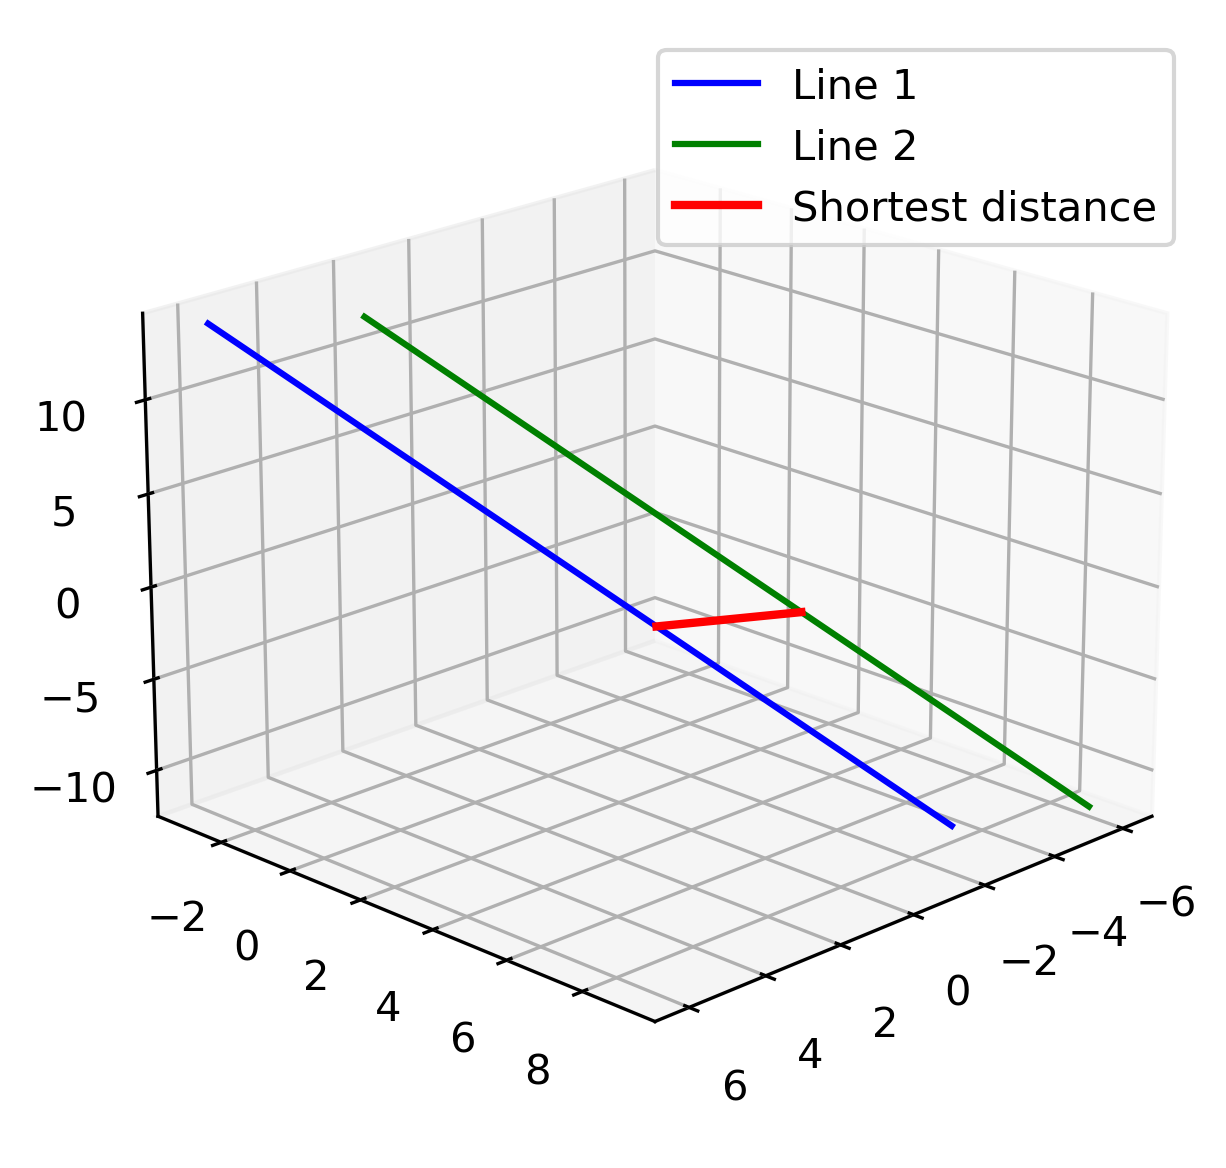
\includegraphics[width=0.7\linewidth]{figures/shortest_distance.png}
    \caption{Shortest distance between two parallel lines}
    \label{fig:placeholder}
\end{figure}

\end{document}
